\documentclass[letterpaper]{article} % DO NOT CHANGE THIS
\usepackage[submission]{aaai2027}  % DO NOT CHANGE THIS
\usepackage[hyphens]{url}  % DO NOT CHANGE THIS
\usepackage{graphicx} % DO NOT CHANGE THIS
\urlstyle{rm} % DO NOT CHANGE THIS
\def\UrlFont{\rm}  % DO NOT CHANGE THIS
\usepackage{natbib}  % DO NOT CHANGE THIS AND DO NOT ADD ANY OPTIONS TO IT
\usepackage{caption} % DO NOT CHANGE THIS AND DO NOT ADD ANY OPTIONS TO IT
\frenchspacing  % DO NOT CHANGE THIS
\usepackage{booktabs}
\usepackage{amsmath,amssymb,amsthm}
\usepackage{tikz}
\usetikzlibrary{arrows.meta, positioning, fit, backgrounds, calc}
\definecolor{rev}{HTML}{2A78D6}
\definecolor{audit}{HTML}{EB6834}
\definecolor{memc}{HTML}{1BAF7A}
\pdfinfo{
/TemplateVersion (2027.1)
}
\setcounter{secnumdepth}{2}
\newtheorem{proposition}{Proposition}
\newcommand{\game}[1]{\textsc{#1}}
\newcommand{\gone}{g_1}
\newcommand{\gstar}{g^{*}}

\title{Penalties Sized to the Gain: When Do Random Audits Stop\\AI Agents from Over-Using a Shared Resource?}
\author{
    Anonymous Submission
}
\affiliations{
}

\begin{document}
\maketitle

\begin{abstract}
Language-model agents that share a limited resource can take more than their allowance, and an overseer can afford to check only a few of them. We tested when random audits stop such over-use, and whether the penalty that stops a given agent can be predicted before it is deployed. We built an audited commons in which six agents draw on a renewable resource, a reviewer sets each agent's allowance to keep the resource at half capacity, and random audits answer a caught violation with a fine, a memory of the offence, or both. We first used programmed agents in three games, Fishery, Forest and River, and then replaced four of the six fishers with language models from four families in 520 games. With programmed agents, audits reduced harm only through their consequences, and deterrence began where the expected fine equalled the gain from cheating; we predicted this threshold in advance in 5 of 5 new settings. Tightening everyone's allowance to absorb known cheaters made cheating pay more than no audits, and aiming each audit at the largest report caught 25\% of liars, against 100\% under random audits. The two language models that over-took on purpose stopped at the fine we predicted in advance from their one-round gain: exactly for Nemotron 3 Super, and one grid step early for gpt-oss-120b. Over-taking rarely paid over the whole game, yet both models continued until the fine outweighed the gain of the round. A reviewer that remembered past over-takes removed most of the harm without any fine, but did not stop the over-taking. Overseers of language-model agents should therefore set penalties against the immediate gain, keep audits random, and use memory where penalties are unavailable.
\end{abstract}

% =====================================================================
\section{Introduction}

Language-model agents increasingly act together on shared, limited resources, such as compute budgets, energy reserves and the economic and natural commons that their users depend on \citep{piatti2024cooperate,bracale2026draining}. An overseer of such a system faces a problem that is familiar in economics and new in AI safety: verification is expensive, so only a few actions can be checked \citep{amodei2016concrete,greenblatt2024control}, and an agent that takes more than its share is seen only if it happens to be checked.

Enforcement economics predicts when checking deters a rational offender: an offender complies once the expected penalty, the probability of being caught times the fine, exceeds the gain from offending \citep{becker1968crime,allingham1972income,avenhaus2002inspection}. AI-control studies evaluate audit budgets, but a caught model is shut down, so audits without consequences, memories of past offences and graded fines remain untested \citep{greenblatt2024control,griffin2024games}. Language-model agents in commons games mostly fail to sustain the resource without enforcement \citep{piatti2024cooperate,bracale2026draining}. Enforcement studies with language models either remove violators flagged by a language-model judge \citep{ye2026norm} or compare one fine below and one above break-even in single decisions \citep{okamoto2026why}. Whether random audits deter agents that act repeatedly on a shared resource, and whether the deterring fine can be predicted for a given model, has not been tested.

We ask: (1) which consequences make sparse random audits reduce harm to a shared resource; (2) does deterrence begin where the expected fine equals the gain from cheating, and can that point be predicted in advance; and (3) do language-model agents follow the same threshold, and which gain, that of one round or of the whole game, sets it?

We address these questions with an \emph{audited commons} (Figure~\ref{fig:step}). Each round, six agents request a share of a renewable resource; a reviewer predicts the effect of the requests and grants allowances that keep the resource at half capacity, where it regrows fastest; each agent then chooses what it actually takes; and random audits check a few agents. We first study three games with programmed agents, whose decisions we can derive, and then replace four of the six fishers in Fishery with language models from four families. We froze a protocol before writing the code of each study, dated every amendment, and report every failed prediction.

% =====================================================================
\section{Related Work}
\label{sec:related}

Scalable oversight concerns objectives that are ``too expensive to evaluate frequently'' \citep{amodei2016concrete,bowman2022measuring}. AI control evaluates protocols that audit a small share of an untrusted model's outputs, and compares random with suspicion-targeted auditing \citep{greenblatt2024control}; \citet{griffin2024games} model such protocols as games. Monitors that check one agent or one action at a time miss harm that only appears in combination \citep{makins2026multiagent,hu2026local}, and rare random audits can deter AI agents in theory when audit draws cannot be learned in advance \citep{gans2026randomized}.

In commons games, ``all but the most powerful LLM agents fail to achieve a sustainable equilibrium'' \citep{piatti2024cooperate}, language-model collectives drain a shared energy reserve like impatient optimisers \citep{bracale2026draining}, and reasoning models free-ride in public-goods games with sanctions \citep{guzman2025corrupted}. \citet{ye2026norm} enforce norms among language-model agents, including in a fishery, by removing violators and tracking the reliability of reporters. None of these studies varies the audit probability or the fine.

The expected-penalty condition goes back to \citet{becker1968crime} and \citet{allingham1972income}. Inspection games formalise partial verification \citep{avenhaus2002inspection}, records of past offences give enforcement leverage \citep{harrington1988enforcement}, report-based cutoff rules can beat random audits in static settings \citep{reinganum1985income}, and a small fine can act as a price \citep{gneezy2000fine}. Language models comply more when a fine lies above break-even than below it \citep{okamoto2026why}, and deceive more when the perceived risk of getting caught falls \citep{scheurer2023strategic}. We combine these strands in one setting: several agents, a renewable resource, random audits with stated odds, graded fines, memory, and a threshold predicted before it is tested (supplementary Table~S4).

% =====================================================================
\section{Methods}
\label{sec:setting}

\begin{figure*}[t]
  \centering
  \resizebox{0.76\textwidth}{!}{% Figure 1: one step of the audited commons game (TikZ, vector). Input inside a figure environment.
% Colours: agents grey, reviewer blue, audits orange (same mapping as the data figures).
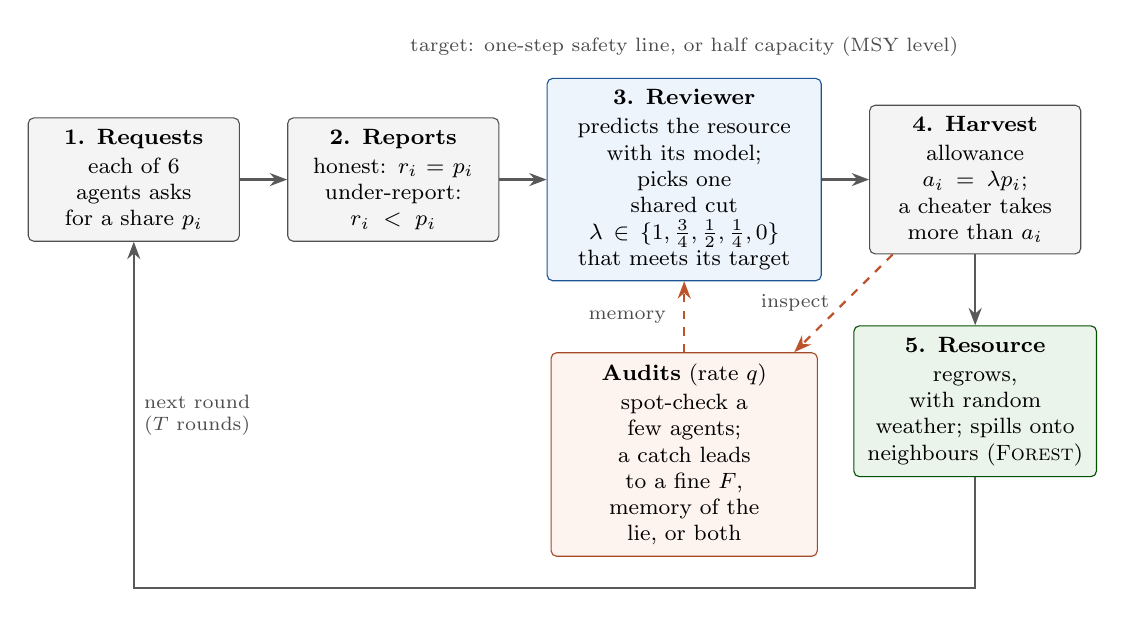
\begin{tikzpicture}[
    font=\footnotesize,
    >={Stealth[length=2.2mm]},
    box/.style={draw=#1!70!black, fill=#1!8, rounded corners=2pt, align=center, inner sep=4pt, minimum height=11mm, text width=24mm},
    lab/.style={font=\scriptsize, align=center, text=black!70},
    flow/.style={->, thick, draw=black!65},
    fb/.style={->, thick, draw=audit!80!black, dashed},
  ]
  \colorlet{agentc}{black!55}
  \colorlet{revc}{rev}
  % ---- row of the step
  \node[box=agentc] (req) {\textbf{1. Requests}\\[1pt] each of 6 agents asks\\ for a share $p_i$};
  \node[box=agentc, right=6mm of req] (rep) {\textbf{2. Reports}\\[1pt] honest: $r_i=p_i$\\ under-report: $r_i<p_i$};
  \node[box=revc, right=6mm of rep, text width=32mm] (rv) {\textbf{3. Reviewer}\\[1pt] predicts the resource\\ with its model; picks one\\ shared cut $\lambda\in\{1,\tfrac34,\tfrac12,\tfrac14,0\}$\\ that meets its target};
  \node[box=agentc, right=6mm of rv] (ex) {\textbf{4. Harvest}\\[1pt] allowance $a_i=\lambda p_i$;\\ a cheater takes\\ more than $a_i$};
  \node[box=green!45!black, below=9mm of ex, text width=28mm, minimum height=17mm] (res) {\textbf{5. Resource}\\[1pt] regrows, with random\\ weather; spills onto\\ neighbours (\textsc{Forest})};
  \node[box=audit, below=9mm of rv, text width=31mm, minimum height=17mm] (au) {\textbf{Audits} (rate $q$)\\[1pt] spot-check a few agents;\\ a catch leads to a fine $F$,\\ memory of the lie, or both};
  % ---- arrows
  \draw[flow] (req) -- (rep);
  \draw[flow] (rep) -- (rv);
  \draw[flow] (rv) -- (ex);
  \draw[flow] (ex) -- (res);
  \draw[flow] (res.south) |- ([yshift=-4mm]au.south) -| (req.south) node[pos=0.75, lab, right] {next round\\ ($T$ rounds)};
  \draw[fb] ([xshift=3mm]ex.south west) -- ([xshift=-3mm]au.north east) node[midway, lab, left=0.5mm] {inspect};
  \draw[fb] (au.north) -- (rv.south) node[midway, lab, left=1mm] {memory};
  % ---- target annotation
  \node[lab, above=1.5mm of rv] {target: one-step safety line, or half capacity (MSY level)};
\end{tikzpicture}
}\\[3mm]
  \resizebox{0.66\textwidth}{!}{% Figure: how harm connects the agents in each game (TikZ, vector). Same colours as Figure 1:
% agents grey, resource green, harm and coupling orange, reviewer blue. Requires \definecolor{rev}, {audit}.
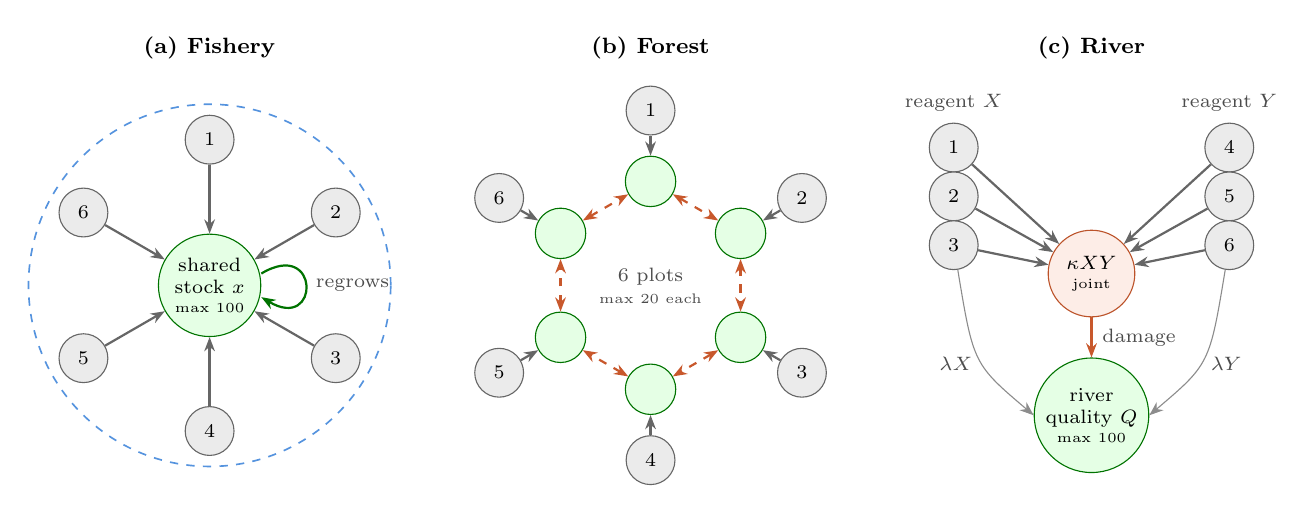
\begin{tikzpicture}[
    font=\footnotesize,
    >={Stealth[length=1.8mm]},
    agent/.style={circle, draw=black!60, fill=black!8, minimum size=6.2mm, inner sep=0pt, font=\scriptsize},
    res/.style={circle, draw=green!45!black, fill=green!10, align=center, inner sep=1pt, font=\scriptsize},
    plot/.style={circle, draw=green!45!black, fill=green!10, minimum size=7.4mm, inner sep=0pt, font=\scriptsize},
    harm/.style={circle, draw=audit!80!black, fill=audit!12, align=center, inner sep=1pt, font=\scriptsize},
    rv/.style={rectangle, rounded corners=2pt, draw=rev!80!black, fill=rev!8, align=center, inner sep=2pt, font=\scriptsize},
    take/.style={->, draw=black!60, thick},
    spill/.style={<->, draw=audit!85!black, thick, dashed},
    cut/.style={draw=rev!70, dashed, thin},
    lab/.style={font=\scriptsize, align=center, text=black!70},
    ttl/.style={font=\footnotesize\bfseries, anchor=south},
  ]
  % ------------------------------------------------------------------ (a) Fishery: a star around one stock
  \begin{scope}[shift={(0,0)}]
    \node[ttl] at (0,2.75) {(a) \textsc{Fishery}};
    \node[res, minimum size=13mm] (S) at (0,0) {shared\\stock $x$\\[-1pt]{\tiny max 100}};
    \foreach \k in {1,...,6} {
      \node[agent] (a\k) at ({90-60*(\k-1)}:1.85) {$\k$};
      \draw[take] (a\k) -- (S);
    }
    \draw[->, draw=green!45!black, thick] ([yshift=1.5mm]S.east) .. controls +(0.75,0.45) and +(0.75,-0.45) .. ([yshift=-1.5mm]S.east)
      node[pos=0.5, lab, right=0pt] {regrows};
    \draw[cut, rev!80, line width=0.6pt] (0,0) circle (2.3);
  \end{scope}
  % ------------------------------------------------------------------ (b) Forest: a ring of plots with spillover
  \begin{scope}[shift={(5.6,0)}]
    \node[ttl] at (0,2.75) {(b) \textsc{Forest}};
    \foreach \k in {1,...,6} {
      \node[plot, minimum size=6.4mm] (p\k) at ({90-60*(\k-1)}:1.32) {};
      \node[agent] (f\k) at ({90-60*(\k-1)}:2.22) {$\k$};
      \draw[take] (f\k) -- (p\k);
    }
    \foreach \k/\j in {1/2,2/3,3/4,4/5,5/6,6/1} {
      \draw[spill] (p\k) -- (p\j);
    }
    \node[lab] at (0,0) {6 plots\\{\tiny max 20 each}};
  \end{scope}
  % ------------------------------------------------------------------ (c) River: two pollutants that harm mainly together
  \begin{scope}[shift={(11.2,0)}]
    \node[ttl] at (0,2.75) {(c) \textsc{River}};
    \foreach \k in {1,2,3} {
      \node[agent] (x\k) at (-1.75,{1.75-0.62*(\k-1)}) {$\k$};
    }
    \foreach \k in {4,5,6} {
      \node[agent] (y\k) at (1.75,{1.75-0.62*(\k-4)}) {$\k$};
    }
    \node[lab] at (-1.75,2.32) {reagent $X$};
    \node[lab] at (1.75,2.32) {reagent $Y$};
    \node[harm, minimum size=11mm] (M) at (0,0.15) {$\kappa XY$\\[-1pt]{\tiny joint}};
    \foreach \k in {1,2,3} {\draw[take] (x\k) -- (M);}
    \foreach \k in {4,5,6} {\draw[take] (y\k) -- (M);}
    \node[res, minimum size=12mm] (Q) at (0,-1.65) {river\\quality $Q$\\[-1pt]{\tiny max 100}};
    \draw[->, draw=audit!85!black, very thick] (M) -- (Q) node[midway, lab, right] {damage};
    \draw[->, draw=black!45, thin] (x3) .. controls (-1.5,-1.0) .. (Q.west) node[pos=0.55, lab, left] {$\lambda X$};
    \draw[->, draw=black!45, thin] (y6) .. controls (1.5,-1.0) .. (Q.east) node[pos=0.55, lab, right] {$\lambda Y$};
  \end{scope}
\end{tikzpicture}
}
  \caption{The audited commons. Top: one round, in which agents request a share and may under-report, the reviewer chooses one shared cut that meets its target, each agent takes its allowance or more, the resource regrows, and random audits answer a caught violation with a fine, a memory of the offence, or both. Bottom: how harm connects the agents in (a) Fishery, where six agents draw on one stock, (b) Forest, where over-cutting a plot damages its two neighbours (dashed), and (c) River, where damage arises mainly where reagents $X$ and $Y$ mix. In every game the reviewer scales all six requests by the same factor; the dashed ring in (a) marks this shared cut, which links every agent to every other.}
  \label{fig:step}
\end{figure*}

\subsection{Audited commons}

$N=6$ agents act for $T$ rounds on a resource with level $x_t\in[0,K]$. After the agents take $c_t=\sum_i c_{i,t}$, the resource regrows logistically,
\begin{equation}
x_{t+1} = y_t + r\,y_t\Bigl(1-\frac{y_t}{K}\Bigr) + \varepsilon_t,\qquad y_t = x_t - c_t,
\label{eq:dyn}
\end{equation}
with weather noise $\varepsilon_t$ in Forest and River. Regrowth $r y(1-y/K)$ peaks at $y=K/2$, where the maximum sustainable harvest $rK/4$ is reached. Agent $i$ requests $p_{i,t}\in[0,\bar c]$ and may report $\hat p_{i,t}\le p_{i,t}$. The reviewer chooses one shared cut $\lambda_t\in\{1,\tfrac34,\tfrac12,\tfrac14,0\}$, the largest whose predicted outcome meets its target, and grants allowances $a_{i,t}=\lambda_t\hat p_{i,t}$. A \emph{joint} reviewer sums all requests before predicting; \emph{local} reviewers judge one request at a time. The target is either a one-step safety line, under which the resource must not fall to a danger level next round, or \emph{half capacity}, $y_t\ge K/2$, the level behind maximum sustainable yield \citep{may1978exploiting}.

We counted a round as \emph{harmful} when the resource fell below half capacity: a Fishery stock below 50 of 100 after fishing, a mean Forest plot health below 10 of 20 (as a 5\% chance constraint), or a River quality below 50 of 100. Following commons-game studies \citep{piatti2024cooperate,perolat2017multiagent}, we also report \emph{efficiency}, the total harvest divided by $T\cdot rK/4$; \emph{equality}, one minus the Gini coefficient of the agents' returns; and \emph{survival}, the share of runs without collapse.

\subsection{Games}

The three games differ in how harm connects the agents (Figure~\ref{fig:step}, bottom). In Fishery, six agents draw on one stock, so each catch lowers what every agent can take in the next round. In Forest, each agent cuts its own plot in a ring of six, and over-cutting a plot damages its two neighbours by 0.12 of the excess each. In River, three agents discharge reagent $X$ and three discharge reagent $Y$; the damage $\kappa XY+\lambda(X+Y)$ arises mainly from the two together, so no single discharge looks harmful on its own. In every game, the reviewer's single shared cut links all six agents.

\subsection{Audits, fines and memory}

An agent \emph{over-takes} when $c_{i,t}>a_{i,t}$ and \emph{under-reports} when $\hat p_{i,t}<p_{i,t}$. Each round, each agent is audited independently with probability $q$, and an audit detects a violation with probability $s$. A caught agent pays a flat fine $F$, so the expected fine per violating round is $e=qsF$. Alternatively, the reviewer keeps a \emph{memory}: it records the caught agent's excess and lowers its later allowances by the mean recorded excess, $a'_{i,t}=\max(0,\lambda_t\hat p_{i,t}-\bar m_i)$.

To predict when a fine deters, let $\gone$ be an agent's gain from one round of over-taking, holding later rounds fixed, and let $\gstar$ be its net gain over complying across the whole game, per round of over-taking.

\begin{proposition}[Break-even]
\label{prop:breakeven}
(i) A risk-neutral agent that maximises each round's catch net of the expected fine over-takes in a round if and only if $e<\gone$; under a flat fine it then takes the maximum $\bar c$. (ii) An agent that commits to one over-take level for the whole game over-takes at some level if and only if $e<\gstar$.
\end{proposition}
\begin{proof}[Sketch]
(i) Over-taking by $\delta>0$ adds $\delta$ to the round's catch and costs $e$ in expectation, independent of $\delta$ under a flat fine; the net gain is largest at the largest $\delta$ and is positive iff $\gone>e$. (ii) A level $d$ yields a total gain $G(d)$ over $n(d)$ over-take rounds and expected fines $e\,n(d)$; it pays iff $G(d)/n(d)>e$, and $\gstar=\max_d G(d)/n(d)$.
\end{proof}

Depleting the resource lowers later catches, so $\gstar\le\gone$ in our games. An agent that decides round by round can therefore keep over-taking at fines where over-taking no longer pays over the game.

\begin{figure*}[t]
  \centering
  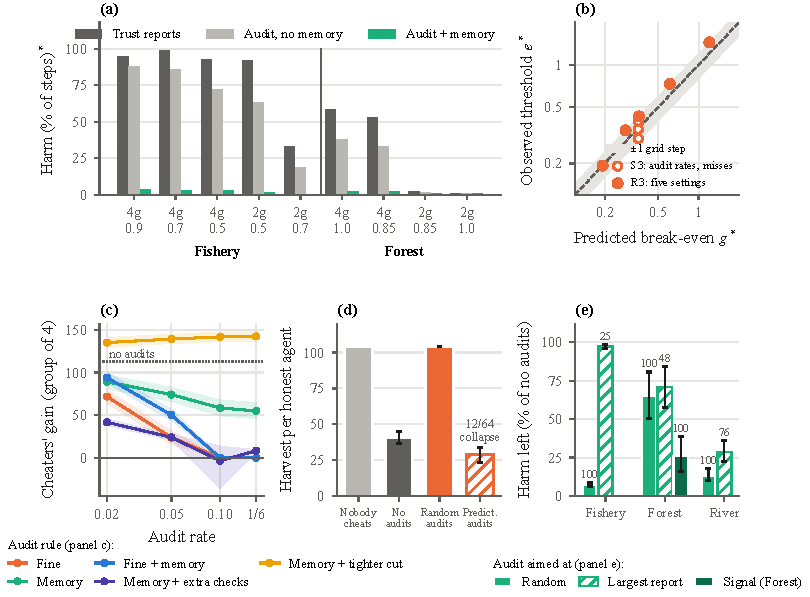
\includegraphics[width=\textwidth]{figures/fig3_audits.pdf}
  \caption{Audits with programmed agents. (a) Share of rounds below the harm line with under-reporters, when nobody is audited, when audits are used without memory, and when the reviewer remembers each caught lie; Fishery and Forest settings differ in the number of greedy agents (2 or 4) and the regrowth rate, and River has three agents per reagent (audits without memory were not run in River). (b) Observed deterrence threshold $e^*$ against the break-even $\gstar$ predicted from runs without audits; filled points are new settings predicted before the search, open points vary the audit rate from $1/6$ to $0.02$ or let audits miss cheats, and the band marks one grid step. (c) Cheaters' gain against the audit rate under five audit rules; the dotted line marks no audits. (d) Harvest per honest agent with a fine of 24 under random audits and audits on a fixed schedule. (e) Harm remaining, relative to no audits, when one audit per round is aimed at a random agent, at the largest report, or at the plot furthest below the reviewer's forecast; numbers give the share of liars ever caught. Error bars and bands show 95\% intervals over populations.}
  \label{fig:audits}
\end{figure*}

\subsection{Programmed agents}

Programmed agents follow threshold rules, and 2 or 4 of the 6 are \emph{greedy}. Misbehaving agents either under-report by a fixed share, or over-take with a level $d\in\{0,\frac14,\frac12,\frac34,1\}$, taking $a+d(p-a)$, which a search chooses to maximise their payoff on 32 training populations. These agents commit to one level per game, as in part (ii) of Proposition~\ref{prop:breakeven}. We evaluated every rule on 64 new populations of 80 rounds.

\subsection{Language-model agents}

In Fishery, with the half-capacity target and 20 rounds, four of the six fishers were language-model agents and two followed fixed rules. Each round, a language-model agent stated a request and, after seeing its allowance, its catch, as JSON in tonnes; it saw the last three rounds of its own history but not the other agents' actions. Audits were independent with $q=1/6$. A catch cost a flat fine $F\in\{0,1,2,4,8,12,18,24,30,36\}$\,t or triggered the reviewer's memory with no fine. The rules stated ``you can choose to catch more than your allowance''; control conditions omitted this sentence or reworded the rules. We counted an over-take when the catch exceeded the allowance by more than 0.06\,t.

We ran gpt-oss-120b, Nemotron 3 Super and Gemma 4 31B, and added Mistral Large 3 as a fourth family, through Ollama Cloud at temperature 0.7 with fixed seeds, on the same 10 populations in every condition. Each model first passed a pilot gate of at least 95\% valid first answers and a mean comprehension score of at least 2 of 3. Across 520 games and 81{,}232 decisions, the models needed no fallback answers and 6 re-prompts, and every comprehension check scored 3 of 3. Before testing fines of 12--30\,t, we froze a prediction of the fine at which gpt-oss-120b and Nemotron 3 Super would stop, derived from their behaviour without a fine.

\subsection{Analysis}

We compared conditions on the same populations and report 95\% paired bootstrap intervals over populations (4{,}000 resamples). Supplementary Table~S1 lists the settings of every study. We mark analyses chosen after the results were seen as post hoc.

% =====================================================================
\section{Results}
\label{sec:results}

\begin{figure*}[t]
  \centering
  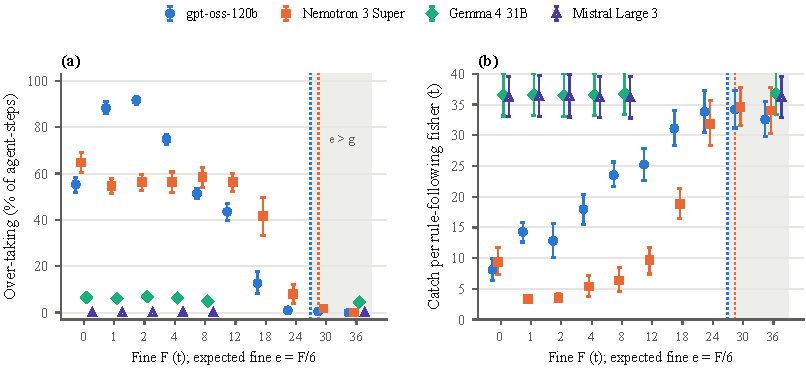
\includegraphics[width=\textwidth]{figures/fig4_llm_main.pdf}
  \caption{Language-model agents in Fishery. (a) Share of rounds in which each model over-took, against the fine $F$ (expected fine $e=F/6$); fines of 12--30\,t were tested for gpt-oss-120b and Nemotron 3 Super only. Dotted lines mark each model's one-round gain $\gone$, and the shaded area marks fines above both. Open triangles: Mistral Large 3, added as a fourth family. (b) Catch of the two rule-following fishers over 20 rounds. Error bars show 95\% intervals over populations.}
  \label{fig:llm}
\end{figure*}

\subsection{Reviewer target and model}

With a joint reviewer and true inputs, the half-capacity target gave a total Fishery harvest of 1{,}393 against 555 under the one-step line (difference $+838$, $[+800,+865]$), because the one-step line let the stock fall to where it regrows slowly. When the reviewer overestimated Forest regrowth by 25\%, its approvals of risky requests rose from 0.9\% to 82\%. Under a hidden collapse point in Fishery, the one-step line collapsed 78\% of populations and the half-capacity target none. A reviewer that learned the model recovered within about 60 rounds (supplementary Figure~S1), as adaptive management in fisheries suggests \citep{ludwig1993uncertainty}.


\subsection{Audit consequences}

Against under-reporters, a reviewer that used audit results only to correct its current decision barely improved safety: unsafe Forest rounds fell from 1.9\% to 1.7\%. Remembering each caught lie removed most of the harm in 9 of 9 Fishery and Forest settings (Figure~\ref{fig:audits}a); in Fishery, unsafe rounds fell from 69\% to 1.5\%. In River, memory reduced the rounds below half capacity from 53\% to 39\%. Memory alone did not deter: adaptive cheaters kept 41\% of their gain even at the highest audit rate, whereas memory plus a fine deterred at an audit rate of 0.05 instead of 0.10.

\subsection{Deterrence threshold with programmed agents}

In the pilot setting, cheaters stopped at $e\approx0.30$--$0.40$, against a predicted break-even of 0.356, for audit rates from $1/6$ to $0.02$ and for audits that missed up to three cheats in four. We then predicted $\gstar$ for five new settings from runs without audits, before any search with fines. In 5 of 5 settings the observed threshold lay within one grid step of the prediction, for predicted thresholds from 0.19 to 1.20 (Figure~\ref{fig:audits}b). A known audit schedule did not deter: honest agents received 28.8 against 40.9 with no audits at all (Figure~\ref{fig:audits}d).

\subsection{Audit rules and audit targeting}

A reviewer that answered known cheaters by lowering the allowance of \emph{all} agents protected the stock but moved the cost onto honest agents. Cheaters gained more than with no audits (142 against 113), and honest agents received 36 each, against 104 under a fine (Figure~\ref{fig:audits}c). Aiming each audit at the largest memory-corrected report kept auditing the same agent: in Fishery, only 25\% of liars were ever caught, against 100\% under random audits, and harm stayed at 96.2\% of rounds against 7.4\%. River showed the same ordering, with 6.0\% against 2.8\% of rounds unsafe and 41\% against 37\% below half capacity. Static models favour report-based cutoff rules \citep{reinganum1985income}; with agents of different sizes playing repeatedly, a rank rule never leaves the largest agent, the feedback loop that \citet{ensign2018runaway} describe for predictive policing. Aiming audits at the plot furthest below the reviewer's forecast gave the least harm in Forest, 26\% of the no-audit level against 65\% at random (Figure~\ref{fig:audits}e).


\begin{figure}[t]
  \centering
  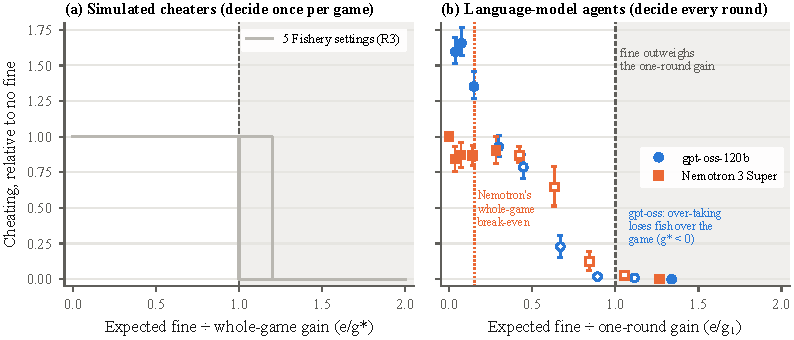
\includegraphics[width=\columnwidth]{figures/fig5_spine.pdf}
  \caption{Observed against predicted stopping fine for the language models. The stopping fine is predicted from each model's one-round gain (filled) or whole-game gain (open), and observed in the threshold test; points on the dashed line are predicted exactly. Vertical whiskers span the last fine that did not deter and the first that did; horizontal whiskers show 95\% intervals of the gain over populations. Grey points: programmed cheaters, predicted from their whole-game gain (Figure~\ref{fig:audits}b). The one-round gain predicted where the language models stopped; their whole-game gain did not.}
  \label{fig:spine}
\end{figure}

\subsection{Language-model agents across fines}

gpt-oss-120b and Nemotron 3 Super over-took in 51--92\% of rounds at every expected fine up to 1.33\,t, and in 0\% at 6\,t (Figure~\ref{fig:llm}a). A small fine raised over-taking by gpt-oss-120b from 55\% to 88--92\%, consistent with a fine acting as a price \citep{gneezy2000fine,okamoto2026why}. Below the threshold the harm was large. Under Nemotron 3 Super, 5 to 10 of 10 lakes collapsed at every fine from 1 to 8\,t, and under gpt-oss-120b the rule-following fishers caught 8--25\,t over the game, against 32--34\,t once over-taking stopped (Figure~\ref{fig:llm}b). Gemma 4 31B over-took in 4--10\% of rounds, almost always by catching its request after the reviewer cut it, and Mistral Large 3 never over-took in 16{,}000 decisions (supplementary Figure~S2); neither model therefore informs the deterrence threshold. A 36\,t fine stopped over-taking under every wording of the rules.

\subsection{Predicted stopping fine}

We measured each model's one-round gain as its mean excess over the allowance on over-take rounds without a fine: $\gone=4.48$\,t for gpt-oss-120b and 4.74\,t for Nemotron 3 Super. We predicted that fines of 12, 18 and 24\,t ($e=2$--$4<\gone$) would not deter and that 30\,t ($e=5>\gone$) would, and then ran 80 games at these fines. Taking ``deterred'' as at most 5\% of rounds at that fine and every larger one, Nemotron 3 Super stopped exactly at 30\,t and gpt-oss-120b one grid step early, at 24\,t (Figure~\ref{fig:llm}a). Over-taking declined gradually rather than in one step: relative to no fine, it was 0.79 and 0.87 at $e/\gone\approx0.45$, 0.23 and 0.65 at $\approx0.65$, and 0.02 and 0.12 at $\approx0.87$ for gpt-oss-120b and Nemotron 3 Super. Our pre-registered expectation that over-taking would stay at or above 25\% at 24\,t failed for both models (1.0\% and 8.0\%).


\subsection{One-round and whole-game gain}

Measured as the programmed cheaters are measured, as the net gain over a compliant game, the whole-game gain per over-take round was $\gstar=-1.05$\,t for gpt-oss-120b, which lost fish by over-taking in 7 of 10 populations because lakes collapsed, and 0.71\,t for Nemotron 3 Super (post hoc). Both models nonetheless kept over-taking until the fine outweighed $\gone$, nearly seven times $\gstar$ for Nemotron 3 Super (Figure~\ref{fig:spine}). The models therefore behaved as in part (i) of Proposition~\ref{prop:breakeven}: they weighed the gain of the round against its expected fine and ignored the depleted stock in later rounds. Two further observations agree with part (i). Over-takes were all-out, reaching the 6\,t maximum in 68\% and 93\% of over-take rounds, as a flat fine gives no reason to take less \citep{stigler1970optimum}. Being caught did not change the next round: gpt-oss-120b over-took again in 78\% of rounds after a caught over-take and 81\% after an unchecked one. Unlike people in some tax experiments, the models did not comply less right after an audit \citep{mittone2006dynamic,kastlunger2009sequences}.

\subsection{Memory and efficiency}

With the reviewer's memory and no fine, over-taking fell to 20\% (gpt-oss-120b) and 33\% (Nemotron 3 Super) of rounds but did not stop. Rounds below half capacity fell from 92\% to 20\% and from 96\% to 40\%, no lake collapsed (against 5 and 1 of 10), and the rule-followers' catch rose from 8 to 29\,t and from 9 to 32\,t. Fines above $\gone$ cost no efficiency: at 30 and 36\,t both models reached 0.99 of the maximum sustainable harvest, kept the stock at or above half capacity in 96--100\% of rounds and gave the most equal outcomes (equality 0.81). Below the threshold, efficiency stayed high only while the stock was over-fished, or fell when it collapsed.

% =====================================================================
\section{Discussion}

\subsection{Penalties and audit design for AI agents}

Our results support one rule for overseeing AI agents on a shared resource: random audits work through their consequences, and a fine deters once its expected value exceeds the gain the agent acts on. For programmed agents that commit to one strategy per game, that gain is the whole-game gain, and runs without audits predict the threshold. For the language models we tested, it is the gain of a single round, which their behaviour without a penalty predicts. Language-model agents in commons are known to neglect the future of the shared stock \citep{piatti2024cooperate,bracale2026draining}; here that neglect set the fine needed to deter them. An overseer should measure the one-round gain, set the expected penalty above it, and keep audits random and covering every agent. Where penalties are unavailable, a memory of past offences protects the resource without deterring. Two shortcuts that save audits, lowering every agent's allowance and aiming audits at the largest report, made matters worse.

\subsection{Limitations and future work}

The language-model results come from one game, two models that over-took on purpose and 10 populations per condition, with one sampled game per population. The fine grid resolves the threshold to about $0.2\,\gone$. Why the models cut back from about $0.4\,\gone$ remains untested: risk aversion \citep{allingham1972income}, a large stated fine read as a warning, and partial attention to the stock all fit. The comparison with the whole-game gain was made after the results. Our ``silent'' control still mentioned a check with a fine of 0\,t, so it did not replicate a no-check condition, and our wording-robustness hypothesis held for Nemotron 3 Super but not for gpt-oss-120b. The programmed cheaters optimise over a one-parameter family, a lower bound on an adaptive adversary. A logging fault lost most saved reasoning texts of the first language-model run; outcomes were unaffected. Varying the audit probability and the fine at a fixed expected penalty would separate risk aversion from myopia, fines that grow with the excess should curb all-out over-taking \citep{stigler1970optimum}, and language-model versions of Forest and River would test whether over-taking spreads along the ring of plots.

\section{Conclusion}

Random audits stopped AI agents from over-using a shared resource only through consequences, only when those consequences reached every agent unpredictably, and only once the expected penalty outweighed the gain the agent acted on. For programmed cheaters that gain was their whole-game gain; for the language models we tested it was the gain of one round. The penalty that stops such agents can be predicted before deployment, and their indifference to the shared stock means that it must be.

\bibliography{refs}

\end{document}
